\section{Discussion}\label{sec:discussion}
% Prompt: Briefly comment on your design specifications, assumptions, shortcomings, and included extra features (if any).
% Highlight any differences between your design and stated specifications.
% Summarize lessons learned while doing the lab and provide advice.

A number of features were added to make development easier and offer a better user experience and interface.

\paragraph{Agnostic LCD configuration routine} When the project board powers on it will load the LCD controller into its default state which includes 8-bit operation.
However, debugging the microcontroller will cause the LCD initialization code to be re-run on an LCD controller that is not in its default state.
This is a particular problem if the LCD initialization assumes that the controller is in 8-bit operating mode because commands will be interpreted differently (perhaps in an undefined manner) in 4-bit mode.

This problem is solved by sending \texttt{0x02} as the initial configuration command.
Recall that the command is sent in two parts: high then low.
In 8-bit mode the high half-word \texttt{0x0} is interpreted as \texttt{0x00} which has no effect on the controller.
The low half-word \texttt{0x2} is interpreted as \texttt{0x20} which sets the controller to 4-bit mode.
If \texttt{0x02} is sent in 4-bit mode it is interpreted correctly as \texttt{0x02} which maps to the command ``send cursor home.'' In both initial states, 8-bit and 4-bit, the controller is operating in 4-bit mode and the rest of the configuration can continue with that assumption.

\paragraph{Custom unit symbols} Instead of displaying the units for resistance as ``Oh'' and frequency as ``Hz'' we use $\Omega$ and a single column character for ``Hz''.
Displaying $\Omega$ was simple because the symbol is pre-loaded in the default $5\times7$ character table (it has address \texttt{0xF4}).

Creating a Hertz symbol was more involved because it's a custom symbol that had to be written into an empty space in the character table.
The HD44780 has 8 spaces in RAM (see Figure~\ref{fig:char-table}) that can can be written to by the programmer.

\begin{figure}[tbph]
  \centering
  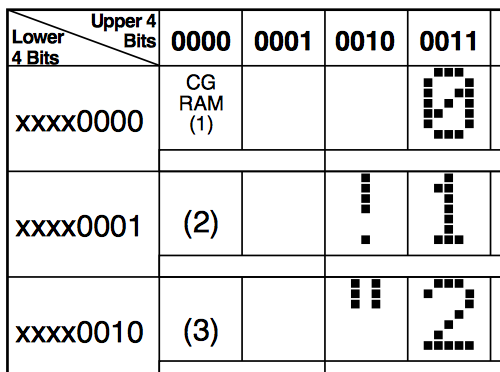
\includegraphics[width=0.4\linewidth]{../graphics/char-table}
  \caption{The first 8 addresses (\texttt{0x00} $\rightarrow$ \texttt{0x07}) in the HD44780 character table are user-writable CGRAM~\cite[p. 17]{H:HD44780}}
  \label{fig:char-table}
\end{figure}

After specifying a CGRAM address, the next 8 words received by the HD44780 will be interpreted as rows of the custom symbol where 1 indicates a dark pixel and 0 a light pixel.
For example, the first row of the custom Hertz symbol in Fig.~\ref{fig:hzsymbol} is sent as a data command with word \texttt{0b10001}.

\begin{figure}[tbph]
  \centering
  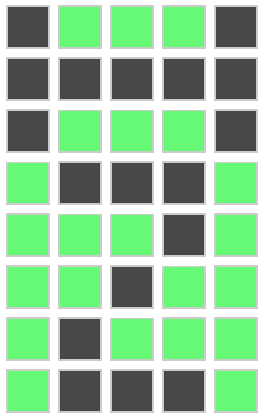
\includegraphics[width=0.2\linewidth]{../graphics/hz_symbol}
  \caption{Custom Hertz symbol}
  \label{fig:hzsymbol}
\end{figure}

The custom symbol is displayed by issuing a word command with the address of the symbol on the character table.
This is the same procedure for displaying other pre-loaded symbols on the table.

\paragraph{Unit auto-ranging} Resistance and frequency units will adjust so that four significant figures are always shown.
The display precision progression is shown in Table~\ref{table:auto-range}.
\begin{table}[htpb]
  \centering
  \caption{Auto-ranging display will always show four significant figures}
  \label{table:auto-range}
  \begin{tabular}{@{}Sr@{}}
    \toprule
    \multicolumn{1}{c}{Measured} & \multicolumn{1}{c}{Displayed} \\ \midrule
    \SI{1.234}{\hertz}       & \texttt{1.234 Hz}                      \\
    \SI{12.34}{\hertz}       & \texttt{12.34 Hz}                      \\
    \SI{123.4}{\hertz}       & \texttt{123.4 Hz}                      \\
    \SI{1234}{\hertz}        & \texttt{1.234kHz}                      \\ \bottomrule
  \end{tabular}
\end{table}
This is implemented with a custom data structure, \texttt{metricFloat}, that holds the scaled value and its associated metric prefix.
\texttt{sprintf} truncates and rounds the scaled value to a fixed precision and creates a \texttt{char[]} that is printed with \texttt{LCD\_SendText()}.
Metric values between 1 and 999,999 can be represented with the appropriate metric prefix and precision.
